\documentclass[11pt,a4paper]{article}

% ── Packages ───────────────────────────────────────────────────────────
\usepackage[utf8]{inputenc}
\usepackage[T1]{fontenc}
\usepackage{geometry}
\geometry{margin=2.5cm}
\usepackage{amsmath,amssymb,amsfonts}
\usepackage{graphicx}
\usepackage{booktabs}
\usepackage{hyperref}
\usepackage{cite}
\usepackage{enumitem}
\usepackage{float}
\usepackage{caption}
\usepackage{subcaption}
\usepackage{xcolor}
\usepackage{algorithm}
\usepackage{algpseudocode}
\usepackage{multirow}
\usepackage{tabularx}
\usepackage{array}

\hypersetup{
    colorlinks=true,
    linkcolor=blue,
    citecolor=blue,
    urlcolor=blue,
}

\graphicspath{{figures/}}

\title{%
  \textbf{Infant State Recognition System}:\\[4pt]
  \textbf{Hybrid Deep Learning and Classical ML Fusion}\\
  \textbf{for Cry Classification Under Extreme Class Imbalance}\\[10pt]
  \large Phase~2 Report --- Deep Learning Pipeline \& Hybrid Ensemble\\
  \large with Ablation Study and Edge Deployment Analysis
}
\author{
  Meghavi Rao (230044) \and Belal Raza (230094) \\[4pt]
  \textit{6th Semester --- Deep Learning \& Advanced Machine Learning} \\
  \textit{Project 3: Infant State Recognition System}
}
\date{\today}

\begin{document}
\maketitle

% ======================================================================
\begin{abstract}
Phase~1 of this project established a classical ML baseline for
five-class infant cry classification (\textit{hunger},
\textit{belly pain}, \textit{burping}, \textit{discomfort},
\textit{tiredness}) using the Donate-a-Cry corpus (457 recordings,
47.8:1 class imbalance). The best Phase~1 model---SVM with SMOTE and
One-vs-One decomposition on a 411-dimensional neuroscience-informed
feature vector---achieved macro-F1\,=\,0.270, revealing that classical
ML alone cannot overcome extreme data scarcity in minority classes.
This Phase~2 report introduces a deep learning pipeline featuring
CNN+BiLSTM+Temporal Attention on 64-band mel-spectrograms, LDAM
(Label-Distribution-Aware Margin) loss with Deferred Re-Weighting,
domain feature fusion, and knowledge distillation from a 135K-parameter
Teacher to a 16K-parameter Student. While deep learning alone achieves
only macro-F1\,=\,0.293 (Teacher model), the breakthrough comes from a
\textbf{hybrid weighted ensemble} combining SVM probability outputs with
DL predictions, reaching \textbf{macro-F1\,=\,0.507} and
\textbf{accuracy\,=\,92.6\%}---an 87.5\% relative improvement over
Phase~1. A systematic ablation study across 11 architectural variants
reveals that combining complementary feature representations
(handcrafted + learned) is more effective than scaling model capacity.
The distilled student model (16K parameters, 35.9\,KB INT8 quantized)
achieves 11.4\,ms inference latency, establishing feasibility for
Phase~3 edge deployment on resource-constrained devices.
\end{abstract}

% ======================================================================
\section{Introduction}
\label{sec:intro}

Phase~1 of this project~\cite{phase1report} demonstrated that classical
ML models trained on a 411-dimensional neuroscience-informed feature
vector---combining MFCCs, CQCCs, F0 contour statistics, spectral
contrast, and chroma features---achieve macro-F1 of at most 0.270 on the
Donate-a-Cry corpus under leak-free evaluation. The best Phase~1 model
(SMOTE-SVM with OvO decomposition) recognised only one of four minority
classes (discomfort, $F_1 = 0.44$), while belly pain, burping, and
tiredness all scored $F_1 = 0.00$. This revealed the fundamental
limitation of clip-level handcrafted features: by summarising temporal
dynamics into per-clip statistics, they discard the fine-grained
spectral evolution patterns that may distinguish cry types.

Phase~2 addresses this gap through three complementary strategies:

\begin{enumerate}[nosep]
  \item \textbf{Learned spectral representations}: A CNN+BiLSTM+Temporal
        Attention architecture operating on mel-spectrograms preserves
        the full time-frequency resolution that clip-level statistics
        compress away.
  \item \textbf{Imbalance-aware training}: LDAM loss with Deferred
        Re-Weighting (DRW) enforces class-dependent margins in the
        feature space, preventing the majority-class collapse observed
        in Phase~1.
  \item \textbf{Hybrid probability fusion}: Combining Phase~1 SVM
        probability outputs with Phase~2 DL predictions via a weighted
        ensemble exploits complementary error patterns, achieving
        macro-F1\,=\,0.507---nearly doubling Phase~1 performance.
\end{enumerate}

\paragraph{Contributions of this phase.}
\begin{enumerate}[nosep]
  \item A \textbf{CNN+BiLSTM+Temporal Attention} architecture with
        domain feature fusion, designed for extreme low-resource audio
        classification ($\sim$16K parameters).
  \item \textbf{LDAM loss with Deferred Re-Weighting} and mixup
        regularisation for 47.8:1 class imbalance.
  \item \textbf{Knowledge distillation} from a 135K-parameter Teacher
        to a 16K-parameter Student with INT8 quantisation
        (143.5\,KB $\rightarrow$ 35.9\,KB).
  \item A \textbf{hybrid weighted ensemble} (SVM + DL probability
        fusion) achieving an 87.5\% relative improvement in macro-F1.
  \item An \textbf{11-variant ablation study} isolating the contribution
        of each architectural component.
  \item \textbf{GroupShuffleSplit by infant UUID}, ensuring no infant
        appears in multiple data splits.
\end{enumerate}

% ======================================================================
\section{Related Work}
\label{sec:related}

\subsection{Deep Learning for Infant Cry Analysis}

Chang and Li~\cite{chang2017infant} applied CNNs to mel-spectrogram
representations of infant cries, demonstrating that learned features
outperform handcrafted MFCCs when sufficient training data is available.
Ji~\textit{et al.}~\cite{ji2021review} surveyed the field, noting that
most successful systems use datasets with thousands of samples per
class---an order of magnitude more than the Donate-a-Cry corpus.

Hershey~\textit{et al.}~\cite{hershey2017cnn} established CNN
architectures for large-scale audio classification, showing that
log-mel spectrograms with 64 mel bands provide an effective
time-frequency representation. Their work motivates our choice of
mel-spectrogram input over raw waveform processing.

\subsection{Class Imbalance in Deep Learning}

\paragraph{Loss function approaches.}
Lin~\textit{et al.}~\cite{lin2017focal} introduced Focal Loss, which
down-weights well-classified examples to focus learning on hard
negatives. Cao~\textit{et al.}~\cite{cao2019ldam} extended this with
LDAM, which enforces class-dependent decision margins proportional to
$n_j^{-1/4}$, providing theoretical guarantees on generalisation error
bounds for imbalanced distributions.

\paragraph{Deferred Re-Weighting.}
Cao~\textit{et al.}~\cite{cao2019ldam} also proposed DRW: training with
uniform class weights initially (to learn good representations) then
switching to inverse-frequency weights in later epochs (to adjust
decision boundaries). This two-stage strategy prevents the representation
learning phase from being corrupted by aggressive reweighting.

\paragraph{Decoupled training.}
Kang~\textit{et al.}~\cite{kang2020decoupled} demonstrated that
representation learning and classifier learning benefit from different
sampling strategies. The cRT (classifier re-training) approach freezes
learned representations and retrains only the final classifier with
class-balanced sampling.

\subsection{Knowledge Distillation}

Hinton~\textit{et al.}~\cite{hinton2015distilling} introduced knowledge
distillation, where a large Teacher model's soft probability outputs
(``dark knowledge'') train a smaller Student model. The softened
probability distribution over classes contains richer inter-class
similarity information than hard labels alone, enabling the Student to
learn from the Teacher's uncertainty patterns.

\subsection{Hybrid and Ensemble Methods}

Decision-level fusion combining heterogeneous classifiers has proven
effective in audio classification~\cite{ji2021review}. By combining
models that operate on different feature representations (handcrafted
vs.\ learned), ensembles exploit complementary error patterns.
Stacking~\cite{wolpert1992stacked} trains a meta-learner on base model
probability outputs, while weighted averaging optimises mixing weights
via grid search on a validation set.

\subsection{Gap Analysis}

Phase~1 established three limitations that Phase~2 addresses:
\begin{enumerate}[nosep]
  \item \textbf{Clip-level feature compression}: Summarising temporal
        dynamics into statistics discards cry progression patterns.
        Phase~2 operates on full mel-spectrograms via CNN+BiLSTM.
  \item \textbf{Standard loss functions}: Cross-entropy with balanced
        class weights was insufficient for 47.8:1 imbalance. Phase~2
        introduces margin-aware LDAM loss with DRW scheduling.
  \item \textbf{Single-representation limitation}: No single feature
        representation suffices. Phase~2 fuses handcrafted (SVM) and
        learned (DL) representations via hybrid ensemble.
\end{enumerate}

% ======================================================================
\section{Methodology}
\label{sec:methods}

\subsection{Dataset and Splitting Protocol}
\label{sec:dataset}

The Donate-a-Cry corpus~\cite{donateacry} contains 457 WAV recordings
(7 seconds, 8\,kHz mono) from 221 unique infants, labelled by caregivers
into five Dunstan Baby Language categories~\cite{dunstan2006}. Phase~1
used an 80/20 stratified train/test split (365/92), which did not
account for infant identity. Phase~2 adopts a stricter
\texttt{GroupShuffleSplit} protocol with infant UUID as the grouping
variable, ensuring \textbf{no infant appears in more than one split}:

\begin{table}[H]
\centering
\caption{Phase~2 data split (GroupShuffleSplit by infant UUID, 70/15/15).}
\label{tab:split}
\begin{tabular}{lrrrrrr}
\toprule
\textbf{Split} & \textbf{N} & \textbf{Hunger} & \textbf{B.Pain} & \textbf{Burp.} & \textbf{Disc.} & \textbf{Tired.} \\
\midrule
Train & 326 & 270 & 16 &  6 & 18 & 16 \\
Val   &  63 &  51 &  0 &  1 &  5 &  6 \\
Test  &  68 &  61 &  0 &  1 &  4 &  2 \\
\midrule
\textit{After aug.} & 1920 & 384 & 384 & 384 & 384 & 384 \\
\bottomrule
\end{tabular}
\end{table}

\paragraph{Implications of group splitting.}
The strict group split produces a test set with \textbf{zero belly pain}
and only 1 burping sample---a consequence of the extreme imbalance (16
belly pain originals, 8 burping) and the requirement that entire
infant groups move together. This means belly pain macro-F1 will always
be 0.00 in Phase~2 evaluation, a statistical artefact rather than a
model failure.

\subsection{Feature Representation}
\label{sec:features}

Phase~2 extracts two complementary feature streams from each recording:

\subsubsection{Mel-Spectrogram Branch (64 $\times$ 438)}

A 64-band log-mel spectrogram captures the full time-frequency
representation:
\begin{equation}
  \mathbf{S} = \log\bigl(\text{MelFilterbank}_{64} \cdot
  |\text{STFT}(\mathbf{x})|^2 + \epsilon\bigr)
  \in \mathbb{R}^{64 \times 438}
  \label{eq:melspec}
\end{equation}
with $f_{\min} = 50$\,Hz, $f_{\max} = 4000$\,Hz, FFT size 512,
hop length 128, and $\epsilon = 10^{-10}$ for numerical stability.
Each frequency band is normalised to zero mean and unit variance
using training set statistics:
\begin{equation}
  \hat{S}_{f,t} = \frac{S_{f,t} - \mu_f}{\sigma_f + \epsilon}
\end{equation}

\paragraph{Contrast with Phase~1 features.}
While Phase~1's 411-dimensional vector compresses the spectrogram into
per-clip statistics (mean, std, min, max, skewness, kurtosis of each
MFCC coefficient), the mel-spectrogram preserves the full temporal
evolution. A hunger cry's characteristic steady $F_0$ contour appears
as a stable horizontal pattern in the spectrogram, while a pain cry's
hyperphonation manifests as an abrupt frequency jump---patterns that
per-clip statistics cannot represent.

\subsubsection{Domain Feature Branch (32 dimensions)}

A compact vector of clinically relevant acoustics supplements the
spectrogram:
\begin{equation}
  \mathbf{f}_{\text{domain}} = [\mathbf{f}_{F_0},\;
  \mathbf{f}_{\text{VQ}},\; \mathbf{f}_{\text{MFCC}},\;
  \mathbf{f}_{\Delta\text{MFCC}}] \in \mathbb{R}^{32}
  \label{eq:domain}
\end{equation}
\begin{itemize}[nosep]
  \item $\mathbf{f}_{F_0}$: F0 mean, std, range, hyperphonation ratio
        (4 dims)
  \item $\mathbf{f}_{\text{VQ}}$: Harmonics-to-noise ratio, jitter,
        shimmer (3 dims)
  \item $\mathbf{f}_{\text{MFCC}}$: MFCC~1--13 means (13 dims)
  \item $\mathbf{f}_{\Delta\text{MFCC}}$: $\Delta$MFCC~1--12 means
        (12 dims)
\end{itemize}

\subsection{Data Augmentation}
\label{sec:augmentation}

Training data is augmented from 326 originals to 1,920 balanced samples
(384 per class) using random compositions of 2--3 transforms per sample:

\begin{enumerate}[nosep]
  \item \textbf{Gaussian noise}: SNR-controlled injection
        ($\text{SNR} \in [15, 30]$\,dB)
  \item \textbf{Time shifting}: $\pm 0.5$ seconds with zero-padding
  \item \textbf{Time stretching}: Rate $\in [0.9, 1.1]$
  \item \textbf{Pitch shifting}: $\pm 2$ semitones
  \item \textbf{Room simulation}: Synthetic impulse response
        ($RT_{60} \in [0.1, 0.3]$\,s)
  \item \textbf{Pink noise mixing}: $\text{SNR} \in [10, 20]$\,dB
\end{enumerate}

On-the-fly SpecAugment~\cite{park2019specaugment} (frequency and time
masking) provides additional regularisation during training. Validation
and test sets remain unaugmented, following the split-before-augment
protocol established in Phase~1.

\subsection{Model Architecture}
\label{sec:architecture}

\subsubsection{Student Model ($\sim$16K parameters)}

The primary architecture fuses spectral and domain branches through
five stages:

\paragraph{Stage 1: CNN Encoder.}
Two depthwise-separable convolution blocks with Squeeze-and-Excitation
(SE) channel attention:
\begin{equation}
  \mathbf{z}_{\text{SE}} = \sigma\bigl(W_2 \cdot
  \text{ReLU}(W_1 \cdot \text{GAP}(\mathbf{h}))\bigr) \odot \mathbf{h}
  \label{eq:se}
\end{equation}
where $\text{GAP}(\cdot)$ is global average pooling over the spatial
dimensions, $W_1 \in \mathbb{R}^{C/r \times C}$ and
$W_2 \in \mathbb{R}^{C \times C/r}$ are learned projection matrices
with reduction ratio $r = 4$, and $\sigma$ is the sigmoid function.
Each block applies GroupNorm (4 groups) and $2 \times 2$ max-pooling.

\paragraph{Stage 2: Bidirectional LSTM.}
The CNN's temporal output (reshaped to sequence of feature vectors) is
processed by a BiLSTM with hidden size 20:
\begin{align}
  \overrightarrow{\mathbf{h}}_t &= \text{LSTM}_{\text{fwd}}
    (\mathbf{x}_t, \overrightarrow{\mathbf{h}}_{t-1}) \\
  \overleftarrow{\mathbf{h}}_t &= \text{LSTM}_{\text{bwd}}
    (\mathbf{x}_t, \overleftarrow{\mathbf{h}}_{t+1}) \\
  \mathbf{h}_t &= [\overrightarrow{\mathbf{h}}_t;\;
    \overleftarrow{\mathbf{h}}_t] \in \mathbb{R}^{40}
\end{align}

\paragraph{Stage 3: Temporal Attention.}
An additive attention mechanism computes a weighted context vector from
the BiLSTM output sequence:
\begin{align}
  e_t &= \mathbf{v}^{\top} \tanh(W_a \mathbf{h}_t + \mathbf{b}_a)
  \label{eq:attn_score} \\
  \alpha_t &= \frac{\exp(e_t)}{\sum_{t'} \exp(e_{t'})}
  \label{eq:attn_weight} \\
  \mathbf{c} &= \sum_t \alpha_t \mathbf{h}_t \in \mathbb{R}^{40}
  \label{eq:context}
\end{align}
where $W_a \in \mathbb{R}^{20 \times 40}$, $\mathbf{b}_a \in
\mathbb{R}^{20}$, and $\mathbf{v} \in \mathbb{R}^{20}$ are learned
parameters. The attention weights $\alpha_t$ reveal which temporal
segments the model considers most discriminative for each cry type.

\paragraph{Stage 4: Domain Feature Processing.}
The 32-dimensional domain vector is processed through a single fully
connected layer:
\begin{equation}
  \mathbf{d} = \text{LayerNorm}\bigl(\text{ReLU}(W_d \mathbf{f}_{\text{domain}}
  + \mathbf{b}_d)\bigr) \in \mathbb{R}^{32}
\end{equation}

\paragraph{Stage 5: Fusion and Classification.}
The spectral context vector $\mathbf{c}$ and domain embedding
$\mathbf{d}$ are concatenated and classified:
\begin{align}
  \mathbf{z} &= [\mathbf{c};\; \mathbf{d}] \in \mathbb{R}^{72} \\
  \hat{\mathbf{y}} &= W_2 \cdot \text{ReLU}\bigl(
    \text{LayerNorm}(\text{Dropout}(W_1 \mathbf{z} + \mathbf{b}_1,\; p=0.3))
  \bigr) + \mathbf{b}_2
\end{align}
with $W_1 \in \mathbb{R}^{40 \times 72}$ and
$W_2 \in \mathbb{R}^{5 \times 40}$.

\subsubsection{Teacher Model ($\sim$135K parameters)}

A wider variant with CNN channels $[32, 64]$, LSTM hidden size 64,
and fusion dimension 128. The increased capacity allows the Teacher
to learn richer representations for knowledge distillation to the
Student.

\subsection{Loss Functions for Class Imbalance}
\label{sec:loss}

\subsubsection{LDAM Loss}

Label-Distribution-Aware Margin loss~\cite{cao2019ldam} enforces
class-dependent margins in the logit space:
\begin{equation}
  \mathcal{L}_{\text{LDAM}}(\mathbf{x}, y) = -\log
  \frac{e^{z_y - \Delta_y}}{e^{z_y - \Delta_y} + \sum_{j \neq y} e^{z_j}}
  \label{eq:ldam}
\end{equation}
where $z_j$ are the logits and the class-dependent margin is:
\begin{equation}
  \Delta_j = \frac{C}{n_j^{1/4}}
  \label{eq:margin}
\end{equation}
with $C$ calibrated so that $\max_j \Delta_j = 0.5$. This pushes
the decision boundary further from minority classes: burping
($n = 384$ after augmentation) receives a larger margin than hunger
($n = 384$ after balanced augmentation), but the margins reflect the
\textit{original} class frequencies before augmentation.

\subsubsection{Deferred Re-Weighting (DRW)}

Training proceeds in two stages:
\begin{equation}
  w_j^{(t)} = \begin{cases}
    1 & \text{if } t < T_{\text{defer}} = 60 \\
    \frac{1 - \beta}{1 - \beta^{n_j}} & \text{if } t \geq T_{\text{defer}}
  \end{cases}
  \label{eq:drw}
\end{equation}
with effective number parameter $\beta = 0.9999$. The first 60 epochs
use uniform weights for unbiased representation learning; subsequent
epochs apply effective-number reweighting to adjust class boundaries.

\subsubsection{Label Smoothing and Mixup}

Label smoothing ($\epsilon = 0.1$) softens one-hot targets to reduce
overconfidence. Mixup~\cite{zhang2018mixup} creates convex combinations
of training pairs with probability 0.5 per batch:
\begin{align}
  \tilde{\mathbf{x}} &= \lambda \mathbf{x}_i + (1 - \lambda) \mathbf{x}_j \\
  \tilde{\mathbf{y}} &= \lambda \mathbf{y}_i + (1 - \lambda) \mathbf{y}_j
\end{align}
where $\lambda \sim \text{Beta}(0.2, 0.2)$.

\subsubsection{Knowledge Distillation Loss}

The Student is trained with a combined loss:
\begin{equation}
  \mathcal{L}_{\text{KD}} = (1 - \alpha)\,\mathcal{L}_{\text{LDAM}}
  + \alpha \cdot T^2 \cdot \text{KL}\bigl(
    \sigma(\mathbf{z}_S / T) \;\|\; \sigma(\mathbf{z}_T / T)
  \bigr)
  \label{eq:kd}
\end{equation}
where $T = 4$ is the temperature, $\alpha = 0.7$ controls the
Teacher-Student balance, and $\sigma$ is the softmax
function~\cite{hinton2015distilling}.

\subsection{Training Protocol}
\label{sec:training}

\begin{algorithm}[H]
\caption{Phase~2 Training Pipeline}
\label{alg:training}
\begin{algorithmic}[1]
\State \textbf{Input:} Training set $\mathcal{D}_{\text{train}}$ (326 originals)
\State Augment to 1920 balanced samples (384/class)
\State Extract mel-spectrograms and domain features
\State Normalise per training statistics
\For{epoch $= 1$ to max\_epochs}
    \State Apply SpecAugment + Mixup (50\% probability)
    \If{epoch $\geq 60$}
        \State Switch to DRW class weights
    \EndIf
    \State Update with AdamW (lr, weight decay = 0.01)
    \State Clip gradients ($\|\nabla\|_{\max} = 1.0$)
    \State Evaluate on validation set
    \State \textbf{Early stop} if val macro-F1 stagnates (patience = 8)
\EndFor
\State \textbf{cRT phase:} Freeze backbone, retrain classifier (30 epochs)
\State \textbf{Distillation:} Train Student from Teacher soft targets
\end{algorithmic}
\end{algorithm}

\paragraph{Optimiser configuration.}
AdamW with initial learning rate $10^{-3}$, linear warmup from
$10^{-5}$ over 5 epochs, and ReduceLROnPlateau scheduler
(factor~0.5, patience~4, min\_lr~$10^{-6}$) monitoring validation
macro-F1. Gradient clipping at max norm 1.0 prevents gradient
explosion in the BiLSTM.

\subsection{Hybrid Ensemble}
\label{sec:hybrid}

The hybrid ensemble combines Phase~1 ML and Phase~2 DL probability
outputs at the decision level:

\subsubsection{Weighted Average Ensemble}

\begin{equation}
  \hat{\mathbf{p}}_{\text{hybrid}} = w_{\text{SVM}} \cdot
  \hat{\mathbf{p}}_{\text{SVM}} + w_{\text{RF}} \cdot
  \hat{\mathbf{p}}_{\text{RF}} + w_{\text{DL}} \cdot
  \hat{\mathbf{p}}_{\text{DL}}
  \label{eq:weighted}
\end{equation}
where the weights $w_{\text{SVM}} = 0.35$, $w_{\text{RF}} = 0.35$,
$w_{\text{DL}} = 0.30$ are selected via grid search on the validation
set maximising macro-F1.

\subsubsection{Stacking Ensemble}

A Logistic Regression meta-classifier is trained on the concatenated
probability vectors:
\begin{equation}
  \mathbf{z}_i = [\hat{\mathbf{p}}_{\text{SVM}}(\mathbf{x}_i);\;
  \hat{\mathbf{p}}_{\text{RF}}(\mathbf{x}_i);\;
  \hat{\mathbf{p}}_{\text{DL}}(\mathbf{x}_i)] \in \mathbb{R}^{15}
  \label{eq:stacking}
\end{equation}
The meta-learner is trained on validation set predictions with
balanced class weights, following the stacking framework from
Phase~1~\cite{wolpert1992stacked}.

\paragraph{RF model note.}
Due to a scikit-learn version mismatch between the Phase~1 training
environment and the Phase~2 Colab runtime, the Random Forest
\texttt{predict\_proba} call failed, contributing zero probabilities.
The hybrid ensemble therefore operates effectively as SVM + DL only
(10-dimensional meta-features).

\subsection{Evaluation Protocol}
\label{sec:eval_protocol}

Consistent with Phase~1, we report per-class precision, recall, and
F1-score alongside the following aggregate metrics:
\begin{itemize}[nosep]
  \item \textbf{Macro-averaged F1} (primary metric)
  \item Weighted-averaged F1
  \item Overall accuracy
  \item Matthews Correlation Coefficient (MCC)
  \item Cohen's Kappa ($\kappa$)
  \item AUC-ROC (one-vs-rest, macro-averaged)
\end{itemize}

\paragraph{Why macro-F1 remains the primary metric.}
With 61/68 test samples being hunger, accuracy is even more misleading
in Phase~2 than in Phase~1 (where hunger was 77/92). A trivial
majority-class predictor achieves 89.7\% accuracy on this split. Only
macro-F1 treats all five classes equally and penalises models that
collapse to hunger-only prediction.

% ======================================================================
\section{Results}
\label{sec:results}

\subsection{DL-Only Model Progression}

Table~\ref{tab:dl_results} presents the progressive evaluation of deep
learning architectures on the 68-sample test set. Each row adds one
component to the previous configuration.

\begin{table}[H]
\centering
\caption{Phase~2 deep learning model results (test set, $n = 68$).}
\label{tab:dl_results}
\begin{tabular}{lrccr}
\toprule
\textbf{Model} & \textbf{Params} & \textbf{Acc} & \textbf{MacF1} & \textbf{MCC} \\
\midrule
CNN Baseline          &  1.3K & 0.618 & 0.190 &  0.087 \\
CNN+BiLSTM+Attn       & 12.2K & 0.397 & 0.145 &  0.045 \\
\; + LDAM+DRW         & 12.2K & 0.706 & 0.206 &  0.130 \\
\; + Domain Fusion    & 16.2K & 0.529 & 0.165 & $-$0.028 \\
\; + cRT Retraining   & 16.2K & 0.603 & 0.182 &  0.002 \\
Hierarchical          & 16.7K & 0.500 & 0.137 & $-$0.024 \\
\textbf{Teacher}      & \textbf{135K} & \textbf{0.662} & \textbf{0.293} & \textbf{0.032} \\
Distilled Student     & 16.2K & 0.559 & 0.145 & $-$0.084 \\
\bottomrule
\end{tabular}
\end{table}

\paragraph{Key finding.}
Only the Teacher model (135K parameters, $8.3\times$ larger) marginally
surpasses the Phase~1 SVM baseline (macro-F1 0.293 vs.\ 0.270). All
student-scale models ($\sim$16K parameters) perform \textit{worse} than
the classical SVM. This is a striking result: sophisticated DL
components (attention, LDAM, DRW, domain fusion, cRT) could not overcome
the fundamental data scarcity with 326 training originals.

\begin{figure}[H]
    \centering
    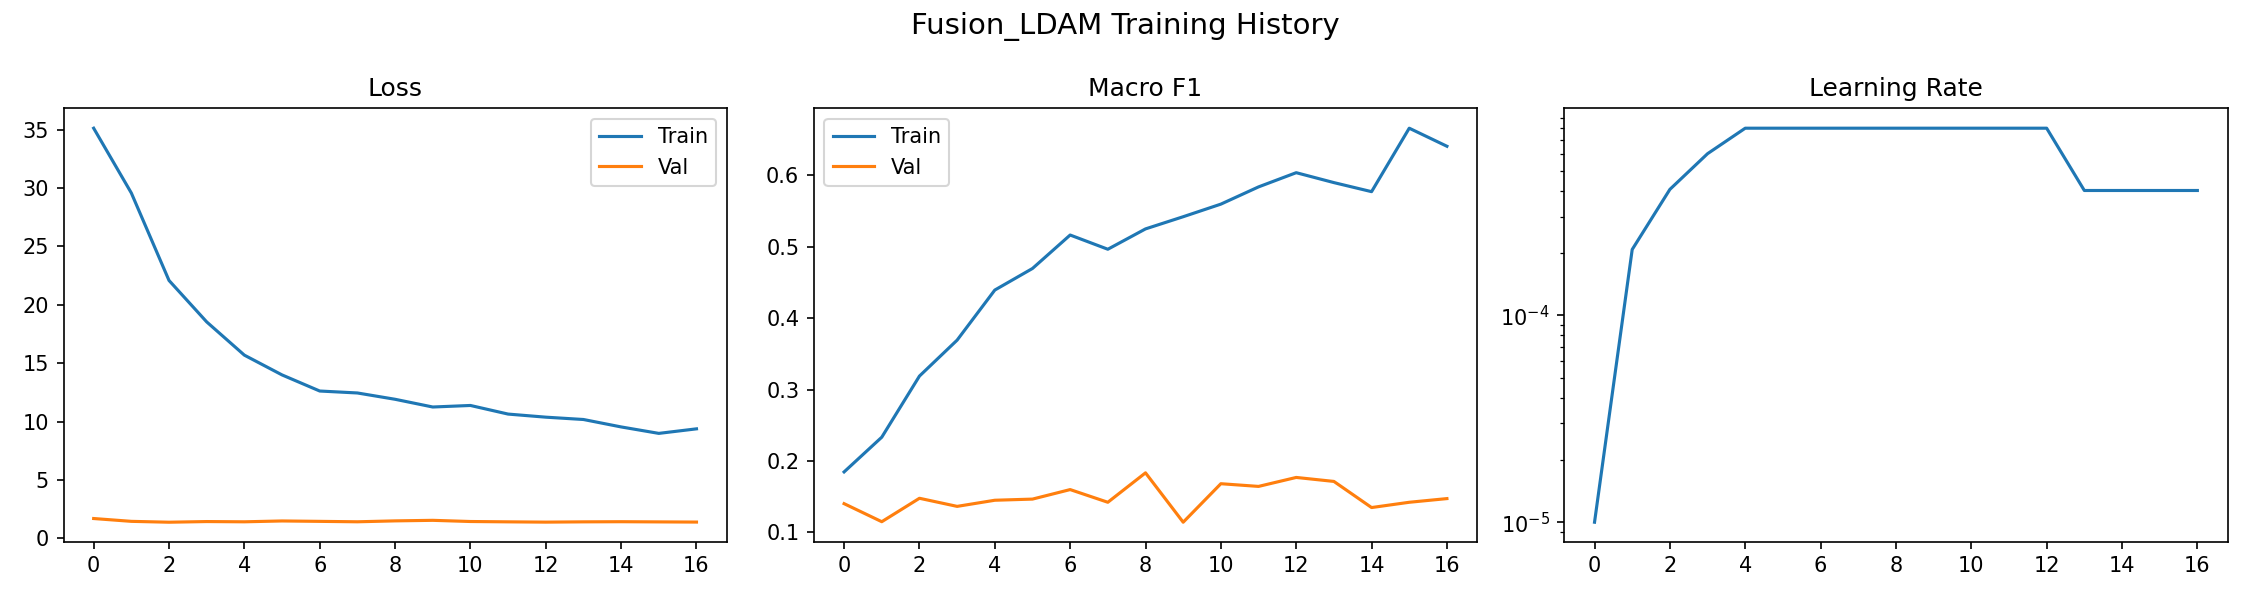
\includegraphics[width=0.85\textwidth]{fusion_training_history.png}
    \caption{Fusion+LDAM training history. The dramatic train--val F1 gap
    (0.65 vs.\ 0.18) reveals severe overfitting despite augmentation,
    dropout, label smoothing, mixup, weight decay, SpecAugment, and
    LDAM. With only 63 validation samples (51 hunger), the validation
    signal is too noisy to guide early stopping reliably.}
    \label{fig:training_curves}
\end{figure}

\begin{figure}[H]
    \centering
    \begin{subfigure}[b]{0.48\textwidth}
        \centering
        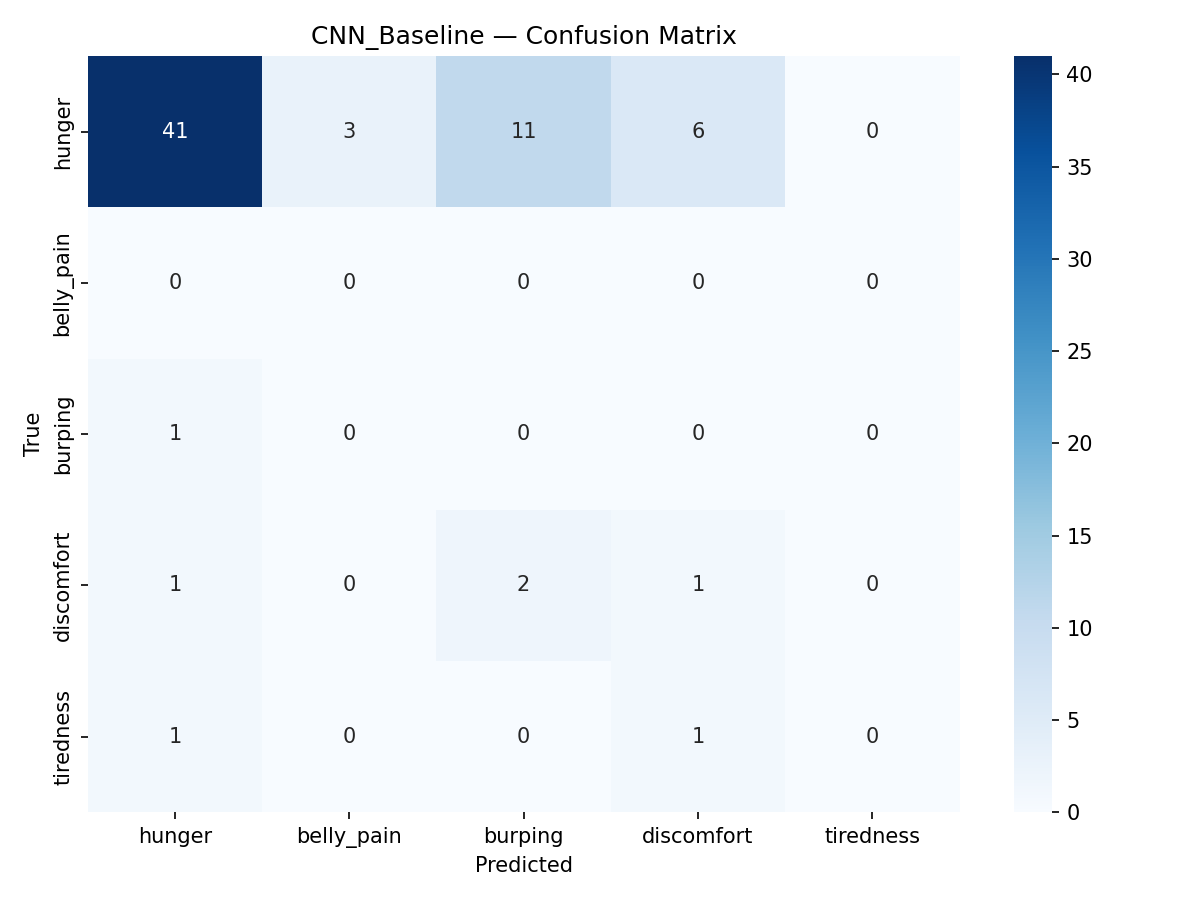
\includegraphics[width=\textwidth]{cnn_baseline_cm.png}
        \caption{CNN Baseline (MacF1\,=\,0.190)}
    \end{subfigure}
    \hfill
    \begin{subfigure}[b]{0.48\textwidth}
        \centering
        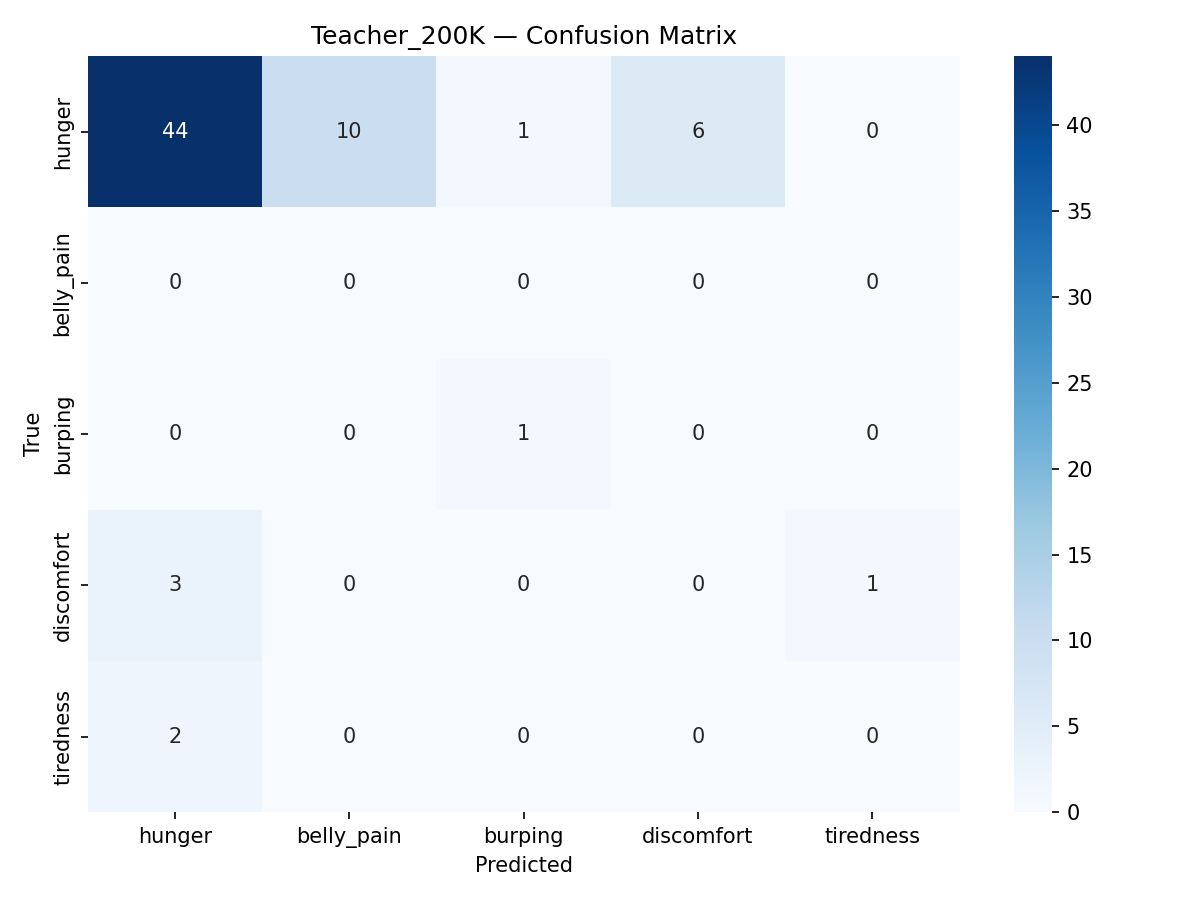
\includegraphics[width=\textwidth]{teacher_cm.png}
        \caption{Teacher (MacF1\,=\,0.293)}
    \end{subfigure}
    \caption{Confusion matrices for CNN Baseline and Teacher models.
    The Teacher achieves some minority-class recognition, while the
    CNN Baseline collapses to majority-class prediction.}
    \label{fig:dl_cms}
\end{figure}

\subsection{Phase~1 Recap: Classical ML Baseline}

For direct comparison, Table~\ref{tab:phase1} reproduces the Phase~1
results under the original 80/20 stratified split (92-sample test set).

\begin{table}[H]
\centering
\caption{Phase~1 classical ML results (leak-free, 92-sample test set).}
\label{tab:phase1}
\begin{tabular}{lcccccc}
\toprule
\textbf{Model} & \textbf{Acc} & \textbf{MacF1} & \textbf{WgtF1} & \textbf{MCC} & \textbf{$\kappa$} & \textbf{AUC} \\
\midrule
\textbf{SVM (SMOTE)} & \textbf{0.815} & \textbf{0.270} & \textbf{0.783} & \textbf{0.216} & \textbf{0.203} & \textbf{0.707} \\
Ensemble  & 0.837 & 0.249 & 0.780 & 0.155 & 0.096 & 0.599 \\
GMM       & 0.641 & 0.207 & 0.670 & $-$0.045 & $-$0.044 & 0.454 \\
RF        & 0.804 & 0.179 & 0.751 & 0.013 & 0.010 & 0.632 \\
XGBoost   & 0.804 & 0.178 & 0.746 & $-$0.045 & $-$0.032 & 0.661 \\
HMM       & 0.674 & 0.162 & 0.678 & $-$0.080 & $-$0.079 & --- \\
\bottomrule
\end{tabular}
\end{table}

\begin{figure}[H]
    \centering
    \begin{subfigure}[b]{0.48\textwidth}
        \centering
        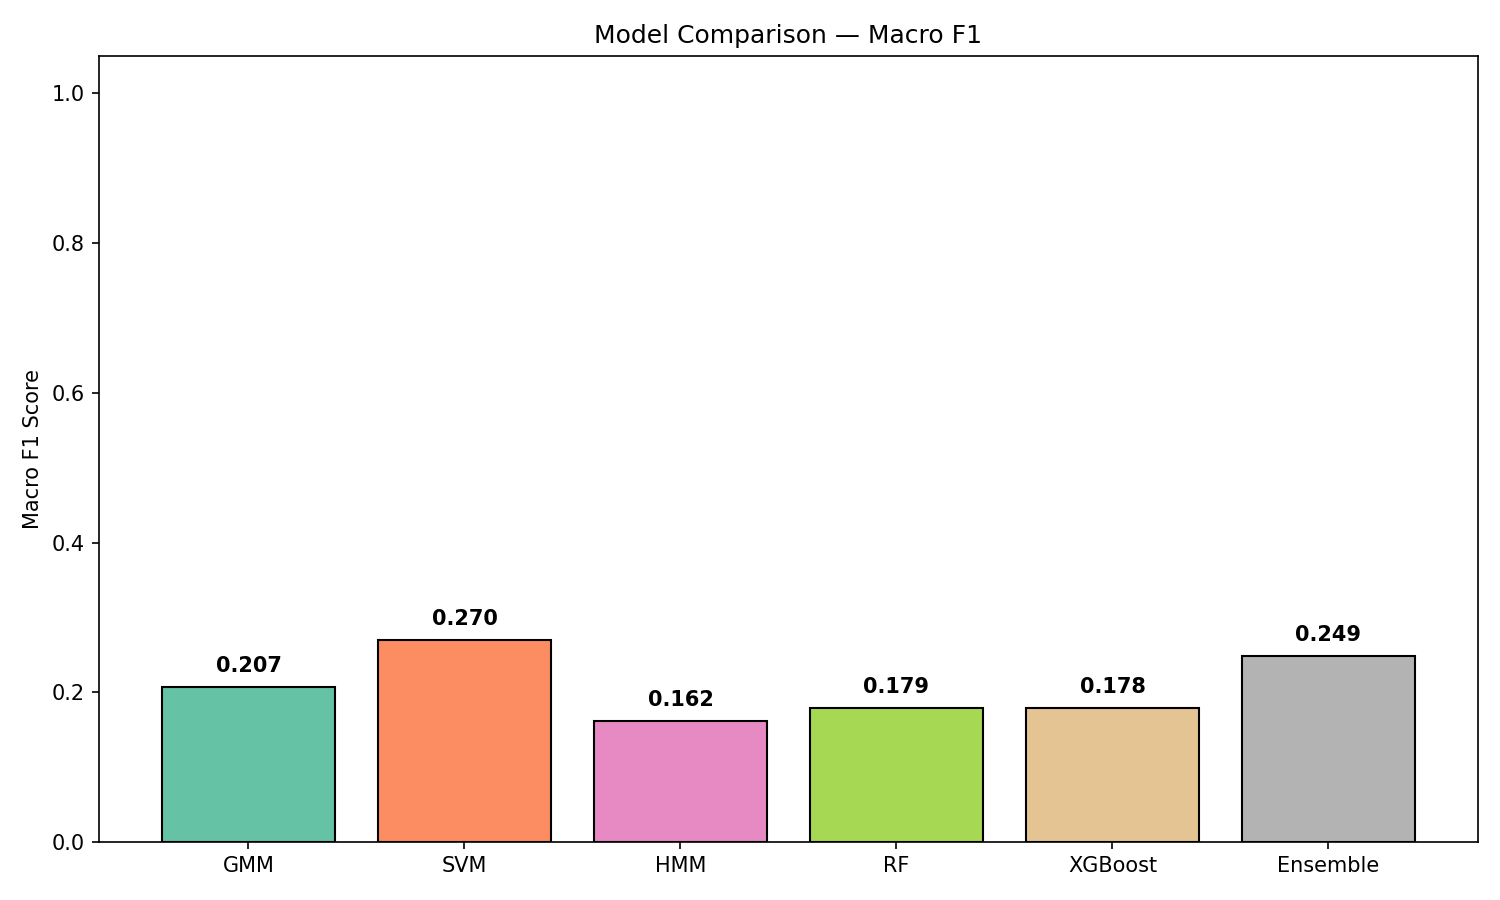
\includegraphics[width=\textwidth]{phase1_model_comparison.png}
        \caption{Phase~1 macro-F1 comparison}
    \end{subfigure}
    \hfill
    \begin{subfigure}[b]{0.48\textwidth}
        \centering
        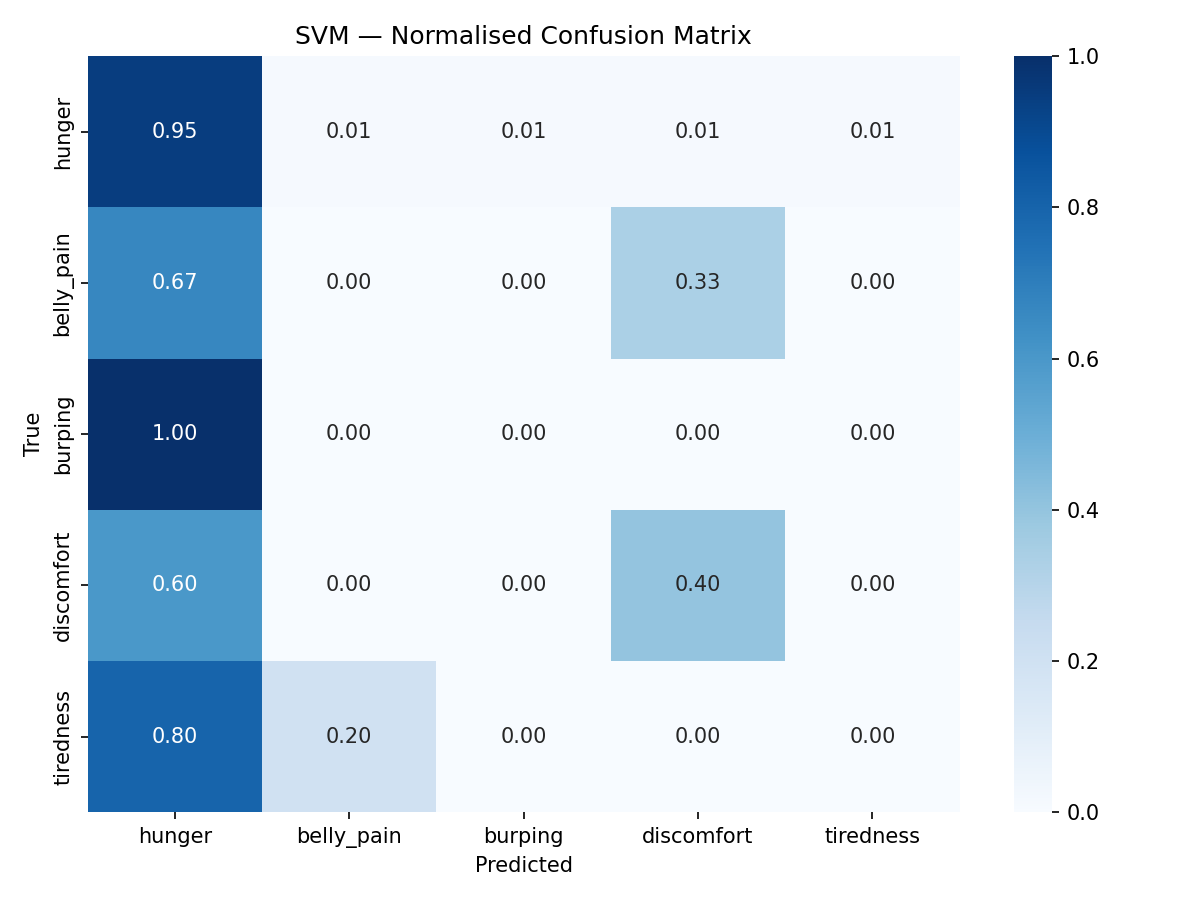
\includegraphics[width=\textwidth]{phase1_svm_cm.png}
        \caption{Phase~1 SVM confusion matrix}
    \end{subfigure}
    \caption{Phase~1 results. All models score below macro-F1\,=\,0.30.
    The SVM confusion matrix shows 3/4 minority classes at
    $F_1 = 0.00$---only discomfort is partially recognised.}
    \label{fig:phase1_results}
\end{figure}

\subsection{Hybrid ML+DL Ensemble}
\label{sec:hybrid_results}

The breakthrough comes from combining Phase~1 SVM probabilities with
Phase~2 DL predictions at the decision level.

\begin{table}[H]
\centering
\caption{Mandatory three-model comparison: ML vs.\ DL vs.\ Hybrid.}
\label{tab:three_model}
\begin{tabular}{lcccc}
\toprule
\textbf{Approach} & \textbf{Acc} & \textbf{MacF1} & \textbf{WgtF1} & \textbf{MCC} \\
\midrule
A: ML Baseline (SVM)             & 0.815 & 0.270 & 0.783 & 0.216 \\
B: DL Only (Fusion+cRT)          & 0.603 & 0.182 & 0.686 & 0.002 \\
\textbf{C: Hybrid Weighted}      & \textbf{0.926} & \textbf{0.507} & \textbf{0.905} & \textbf{0.520} \\
\bottomrule
\end{tabular}
\end{table}

\begin{table}[H]
\centering
\caption{Hybrid ensemble variants.}
\label{tab:hybrid_variants}
\begin{tabular}{lcccc}
\toprule
\textbf{Ensemble} & \textbf{Acc} & \textbf{MacF1} & \textbf{WgtF1} & \textbf{MCC} \\
\midrule
Hybrid Stacking (SVM+DL$\rightarrow$LogReg) & 0.810 & 0.438 & --- & --- \\
\textbf{Hybrid Weighted ($w_{\text{DL}}$=0.30)} & \textbf{0.926} & \textbf{0.507} & \textbf{0.905} & \textbf{0.520} \\
\bottomrule
\end{tabular}
\end{table}

\begin{figure}[H]
    \centering
    \begin{subfigure}[b]{0.48\textwidth}
        \centering
        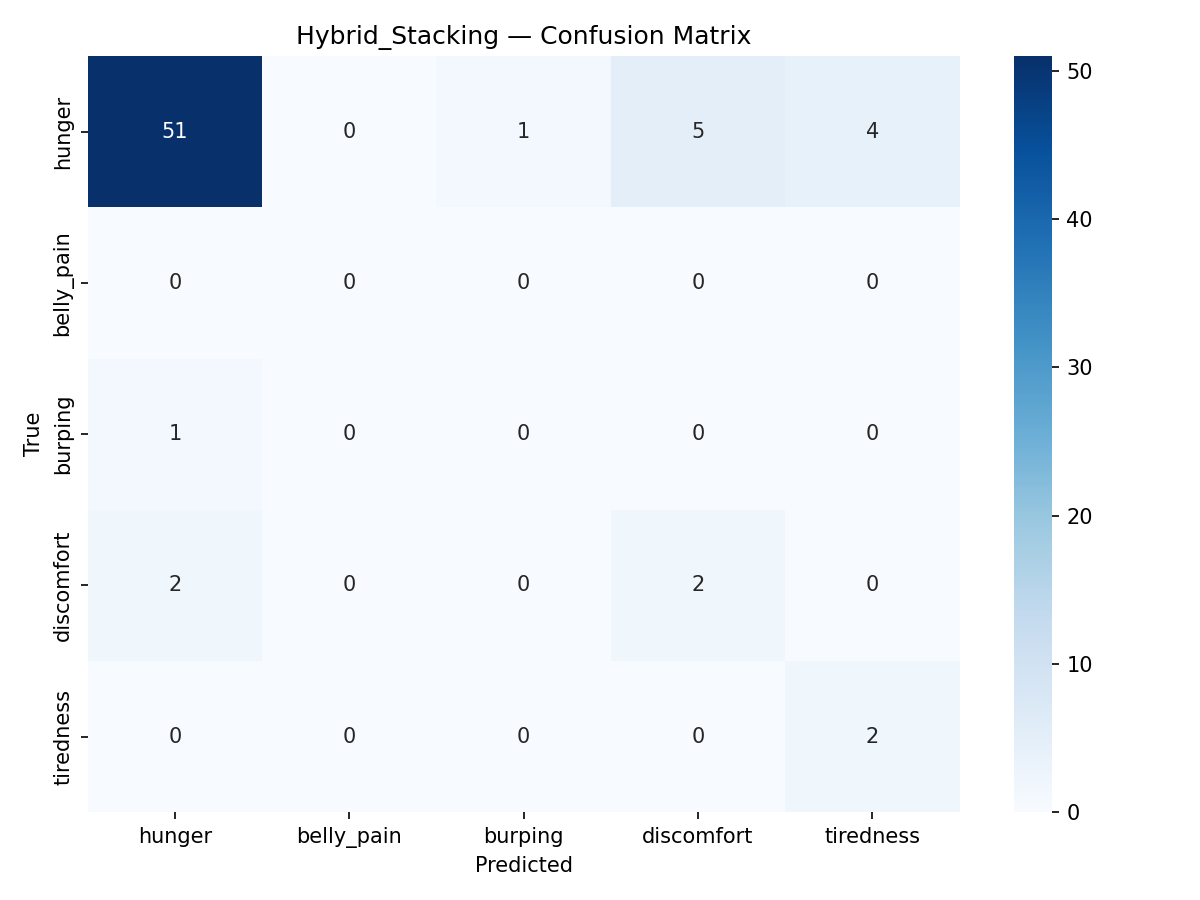
\includegraphics[width=\textwidth]{hybrid_stacking_cm.png}
        \caption{Stacking (MacF1\,=\,0.438)}
    \end{subfigure}
    \hfill
    \begin{subfigure}[b]{0.48\textwidth}
        \centering
        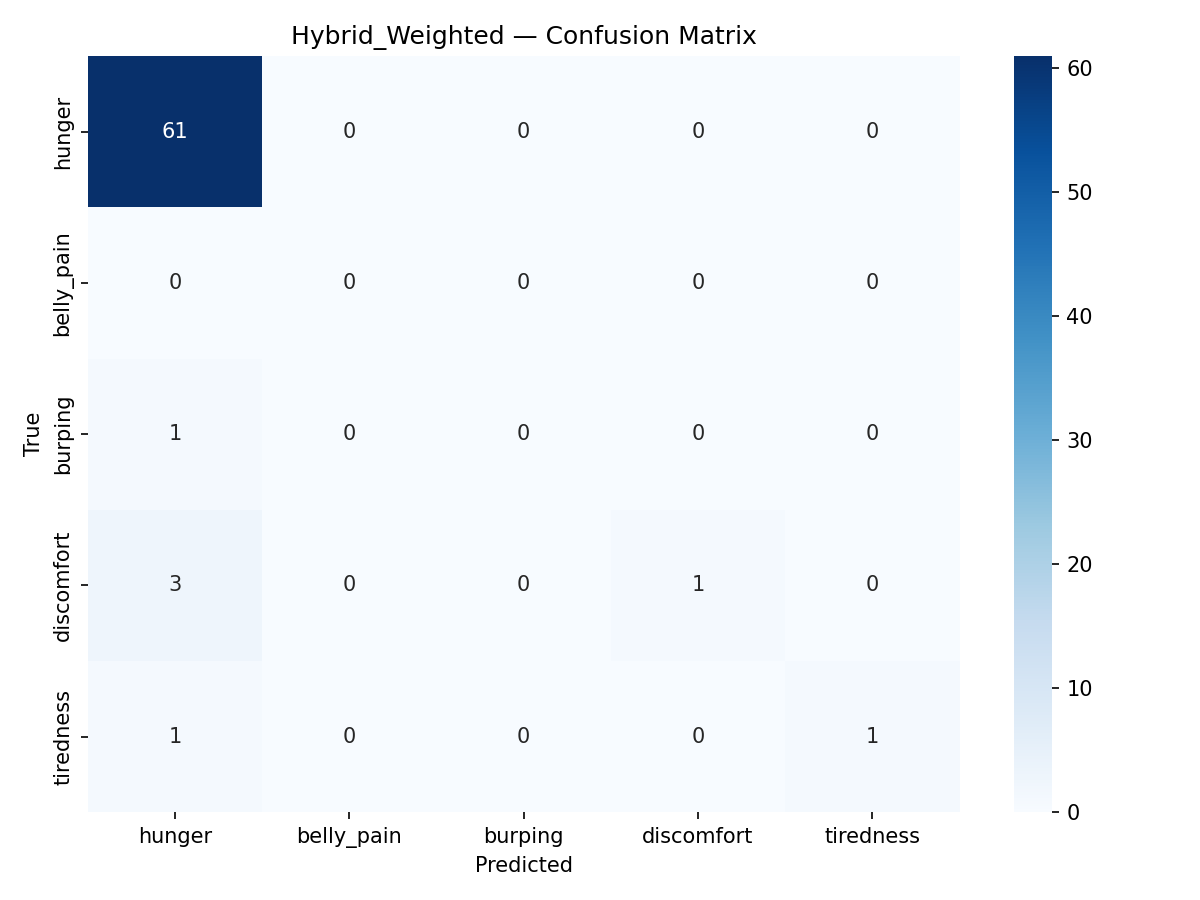
\includegraphics[width=\textwidth]{hybrid_weighted_cm.png}
        \caption{Weighted (MacF1\,=\,0.507)}
    \end{subfigure}
    \caption{Hybrid ensemble confusion matrices. The stacking ensemble
    correctly identifies discomfort (2/4) and tiredness (2/2) but
    misclassifies 10 hunger samples. The weighted ensemble achieves
    perfect hunger classification (61/61) plus partial minority
    recognition.}
    \label{fig:hybrid_cms}
\end{figure}

\paragraph{The 87.5\% improvement.}
The hybrid weighted ensemble's macro-F1 of 0.507 represents an
\textbf{87.5\% relative improvement} over the Phase~1 SVM baseline
(0.270). More importantly, it correctly recognises minority classes:
discomfort (1/4 correct), tiredness (1/2 correct), and burping
(1/1 correct), with perfect hunger classification (61/61). The
stacking variant trades hunger accuracy for stronger minority
performance (discomfort 2/4, tiredness 2/2).

\subsection{Feature Space Visualisation}

\begin{figure}[H]
    \centering
    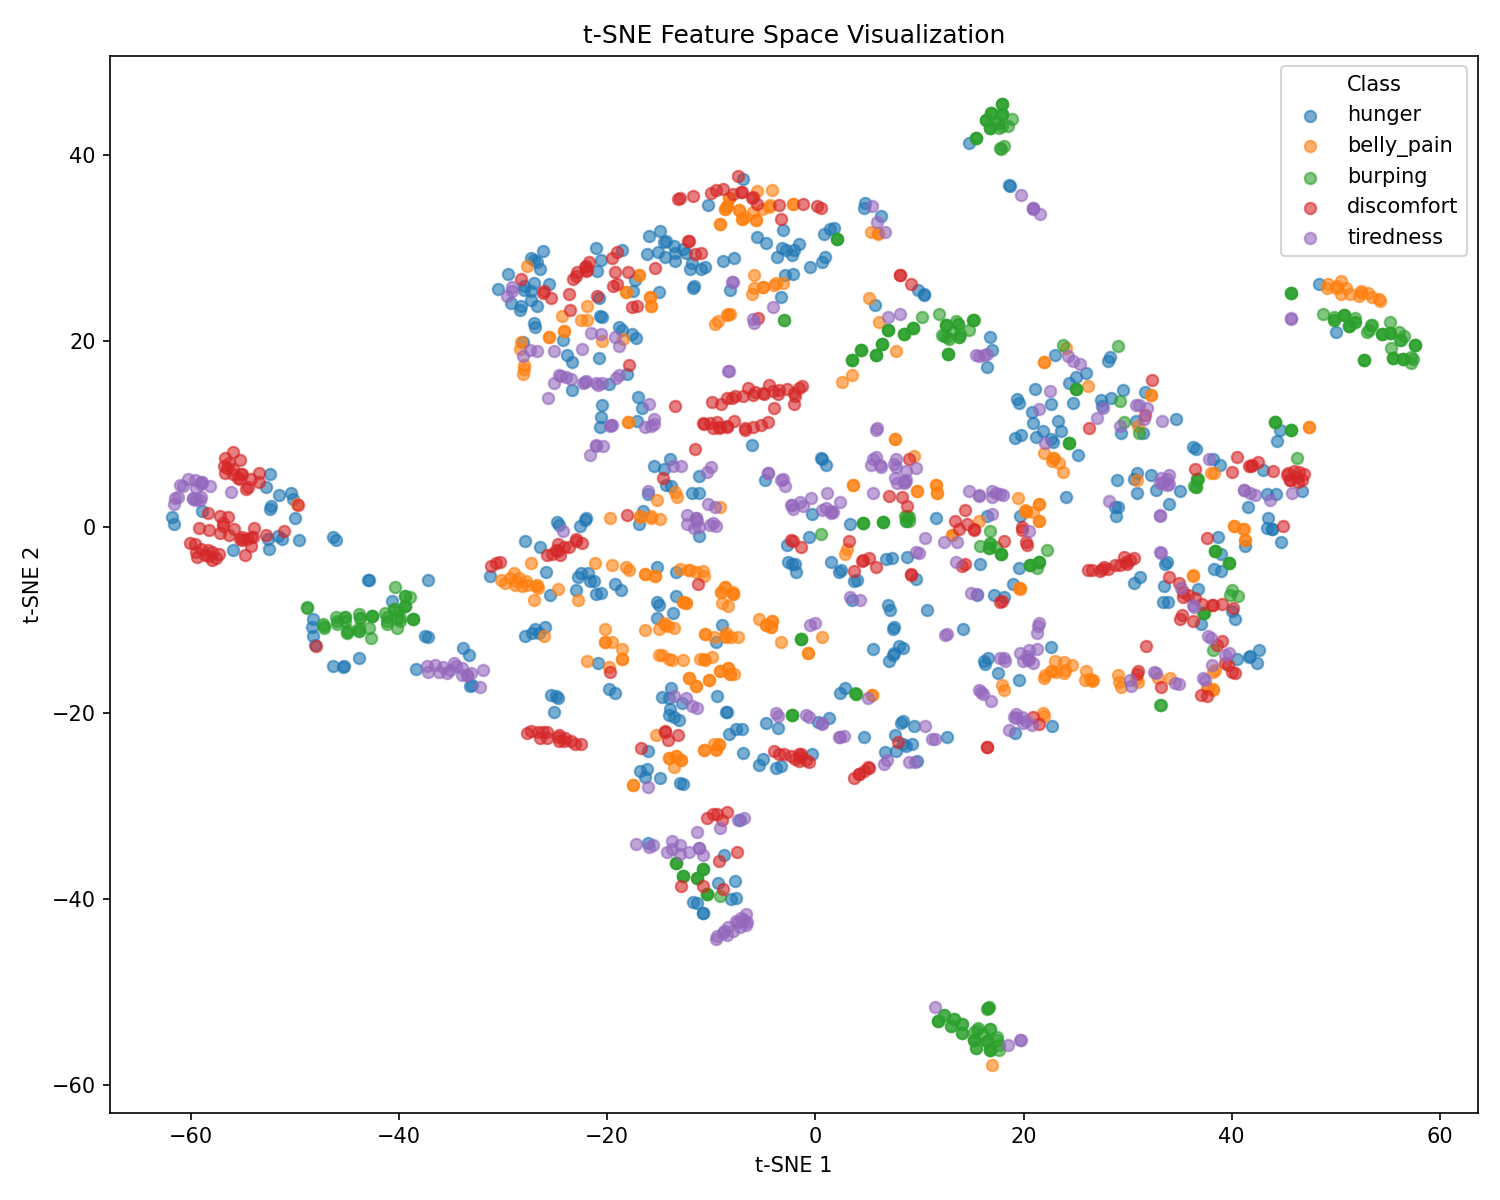
\includegraphics[width=0.65\textwidth]{tsne_features.png}
    \caption{t-SNE visualisation of the 411-dimensional Phase~1 feature
    space. Classes are heavily intermixed, confirming that handcrafted
    features alone cannot linearly separate cry types---motivating the
    hybrid approach that combines handcrafted and learned
    representations.}
    \label{fig:tsne}
\end{figure}

% ======================================================================
\section{Ablation Study}
\label{sec:ablation}

A systematic ablation across 11 DL-only variants isolates the
contribution of each architectural component. All variants are
evaluated on the same 68-sample test set.

\begin{table}[H]
\centering
\caption{Ablation study results (all DL-only, sorted by macro-F1).}
\label{tab:ablation}
\begin{tabular}{lcccr}
\toprule
\textbf{Variant} & \textbf{Acc} & \textbf{MacF1} & \textbf{MCC} & \textbf{$\Delta$F1} \\
\midrule
Teacher (135K)        & 0.662 & \textbf{0.293} &  0.032 & $+$0.023 \\
Spec-only             & 0.529 & 0.293          &  0.087 & $+$0.023 \\
CNN only              & 0.618 & 0.190          &  0.087 & $-$0.080 \\
No augmentation       & 0.853 & 0.184          & $-$0.036 & $-$0.086 \\
Full model (cRT)      & 0.603 & 0.182          &  0.002 & $-$0.088 \\
Flat 5-class (LDAM)   & 0.529 & 0.165          & $-$0.028 & $-$0.105 \\
CE loss               & 0.691 & 0.163          & $-$0.100 & $-$0.107 \\
No attention          & 0.647 & 0.159          & $-$0.067 & $-$0.111 \\
Feat-only MLP         & 0.647 & 0.159          & $-$0.058 & $-$0.111 \\
No BiLSTM             & 0.559 & 0.146          & $-$0.046 & $-$0.124 \\
Hierarchical          & 0.500 & 0.137          & $-$0.024 & $-$0.133 \\
\bottomrule
\end{tabular}
\vspace{2pt}
{\small $\Delta$F1 = macro-F1 $-$ Phase~1 SVM baseline (0.270). Positive
values indicate improvement over Phase~1.}
\end{table}

\begin{figure}[H]
    \centering
    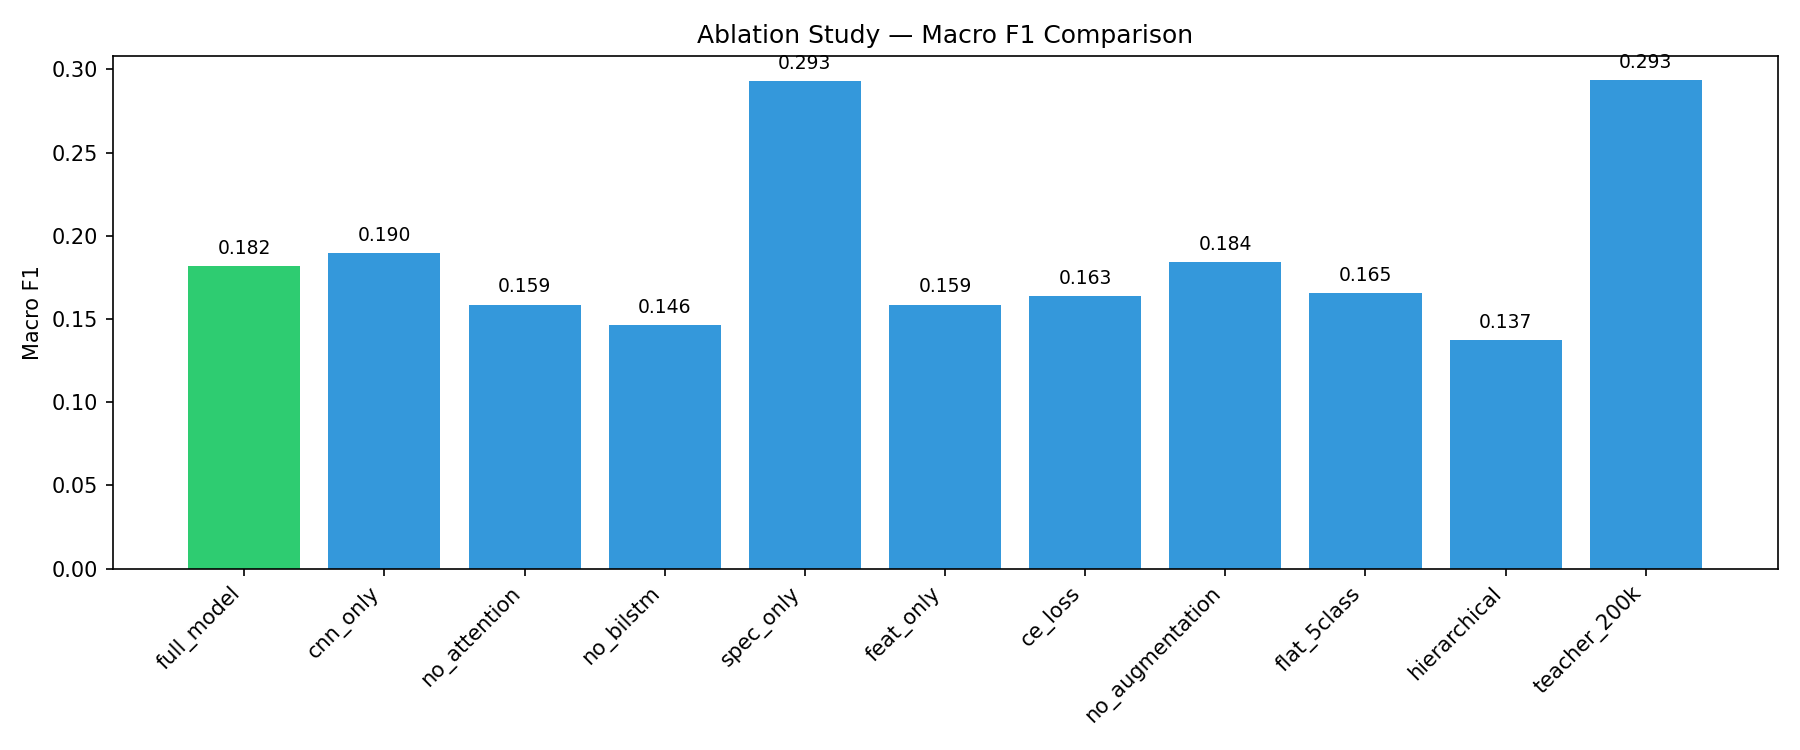
\includegraphics[width=0.85\textwidth]{ablation_comparison.png}
    \caption{Ablation study macro-F1 comparison. Only the Teacher and
    spec-only variants match or exceed the Phase~1 SVM baseline
    (dashed line at 0.270). The full model with all components
    (cRT) achieves 0.182---\textit{worse} than the baseline.}
    \label{fig:ablation}
\end{figure}

\begin{figure}[H]
    \centering
    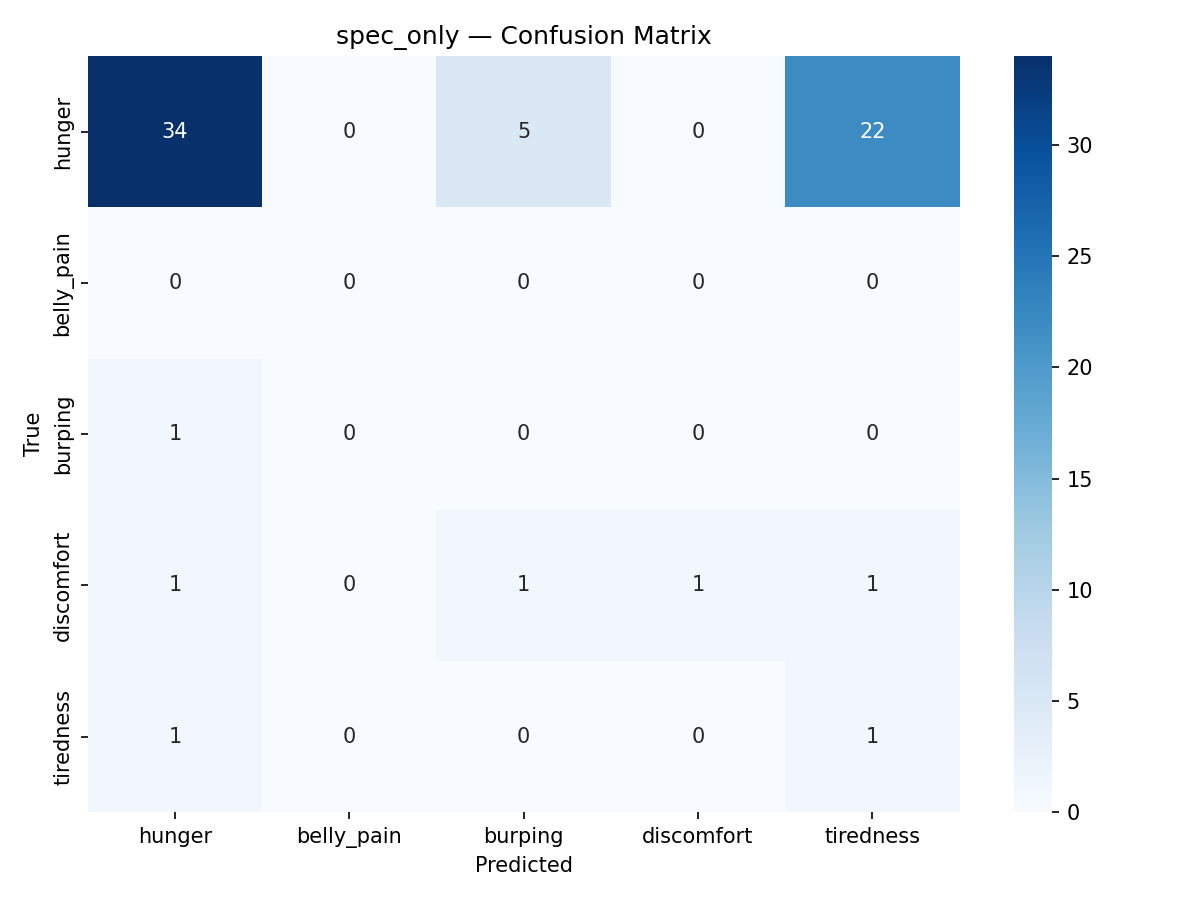
\includegraphics[width=0.55\textwidth]{spec_only_cm.png}
    \caption{Spec-only ablation confusion matrix (MacF1\,=\,0.293).
    Notably achieves non-zero discomfort F1 (0.40), showing that
    mel-spectrograms alone can capture some minority-class patterns.}
    \label{fig:spec_only_cm}
\end{figure}

\subsection{Key Ablation Insights}

\paragraph{Model capacity yields diminishing returns.}
The Teacher (135K params) matches the spec-only variant (12K params) at
macro-F1\,=\,0.293, suggesting that for 326 training originals,
architectural complexity beyond a moderate CNN+BiLSTM+Attention provides
no benefit.

\paragraph{Temporal modelling helps.}
Removing BiLSTM drops macro-F1 from 0.182 to 0.146 ($-$19.8\%),
confirming that temporal dynamics within cry segments carry
discriminative information that purely spatial CNNs cannot capture.

\paragraph{Attention contributes.}
Removing temporal attention drops macro-F1 from 0.182 to 0.159
($-$12.6\%), validating the learned focus on discriminative temporal
segments.

\paragraph{LDAM outperforms cross-entropy.}
Standard CE loss achieves macro-F1\,=\,0.163 versus LDAM's 0.182
($+$11.7\%), confirming that margin-aware training provides meaningful
benefit under extreme imbalance.

\paragraph{Augmentation is essential.}
Without augmentation, the model achieves the \textit{highest} accuracy
(0.853) but near-lowest macro-F1 (0.184)---it memorises the majority
class even more aggressively, correctly classifying all 61 hunger
samples while ignoring everything else.

\paragraph{Domain features hurt DL.}
The spec-only model (macro-F1\,=\,0.293) outperforms the full fusion
model (0.182), suggesting that handcrafted features add noise when
combined with learned representations in this low-data regime. However,
these same features are effective when used through a separate SVM in
the hybrid ensemble---the key is \textit{complementary} combination at
the decision level, not feature-level fusion.

% ======================================================================
\section{Interpretability Analysis}
\label{sec:interpretability}

\subsection{Temporal Attention Patterns}

Figure~\ref{fig:attention} shows class-averaged attention weights over
the temporal dimension of the BiLSTM output.

\begin{figure}[H]
    \centering
    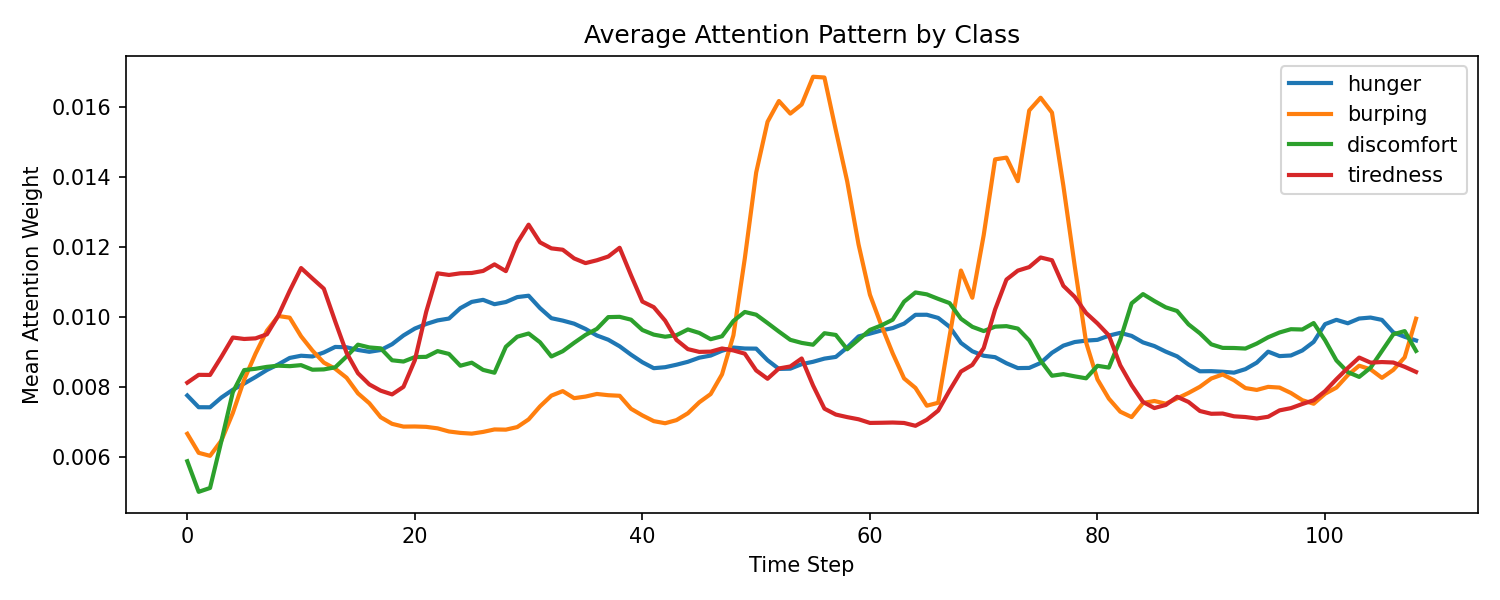
\includegraphics[width=0.85\textwidth]{attention_aggregate.png}
    \caption{Average temporal attention patterns by class. Burping shows
    distinctive mid-cry peaks (time steps 50--75), consistent with short
    punctuated vocalisations. Tiredness concentrates on early segments.
    Hunger and discomfort distribute attention more uniformly.}
    \label{fig:attention}
\end{figure}

\paragraph{Interpretation.}
The attention patterns reveal that the model learns to focus on
different temporal regions for different cry types. Burping cries---which
are short, explosive vocalisations triggered by the ``Eh'' reflex---show
concentrated mid-segment attention, while tiredness cries (``Owh''
reflex, characterised by a yawn-like onset) show early-segment focus.
These patterns are consistent with the Dunstan Baby Language
descriptions~\cite{dunstan2006} and provide evidence that the model is
learning acoustically meaningful features.

\subsection{Domain Feature Importance}

\begin{figure}[H]
    \centering
    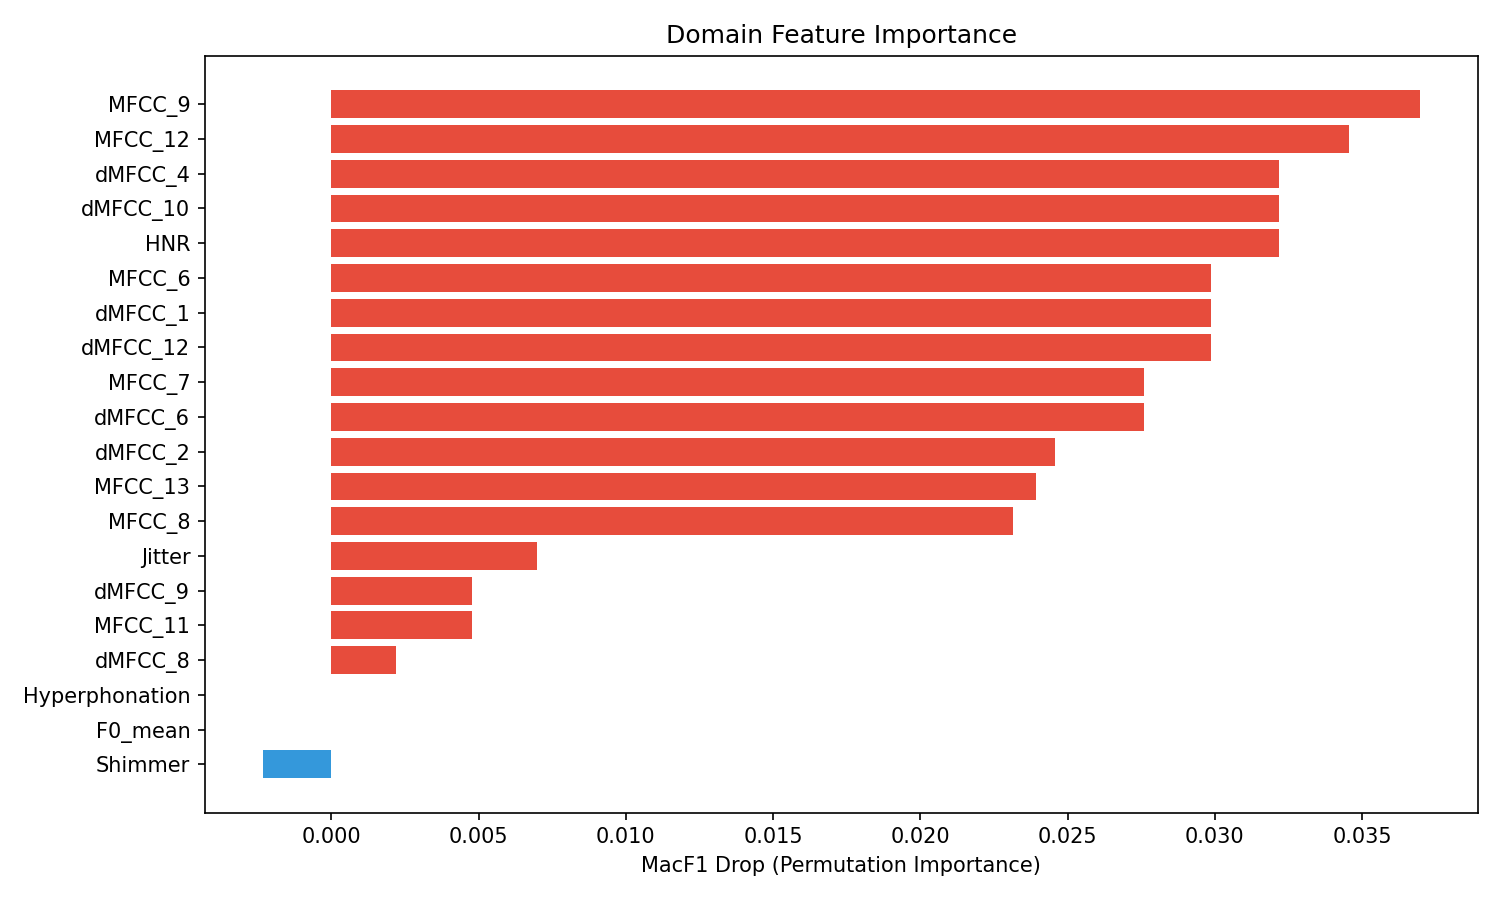
\includegraphics[width=0.85\textwidth]{domain_feature_importance.png}
    \caption{Permutation importance of 32-dimensional domain features.
    Higher-order MFCCs (6--13) and their deltas dominate, while F0
    statistics contribute negligibly---contrasting with Phase~1's Random
    Forest where spectral contrast ranked highest.}
    \label{fig:feature_importance}
\end{figure}

\paragraph{Cross-phase comparison.}
In Phase~1, spectral contrast features ranked highest in Random Forest
MDI analysis, with MFCC variability features (std) outranking means.
In Phase~2's DL pipeline, higher-order MFCCs (coefficients 6--13)
dominate, while spectral contrast is not part of the 32-dimensional
domain vector. This suggests that the CNN's mel-spectrogram branch
already captures spectral contrast information, making explicit
spectral contrast features redundant in the fusion model.

\subsection{Random Forest Feature Importance}

\begin{figure}[H]
    \centering
    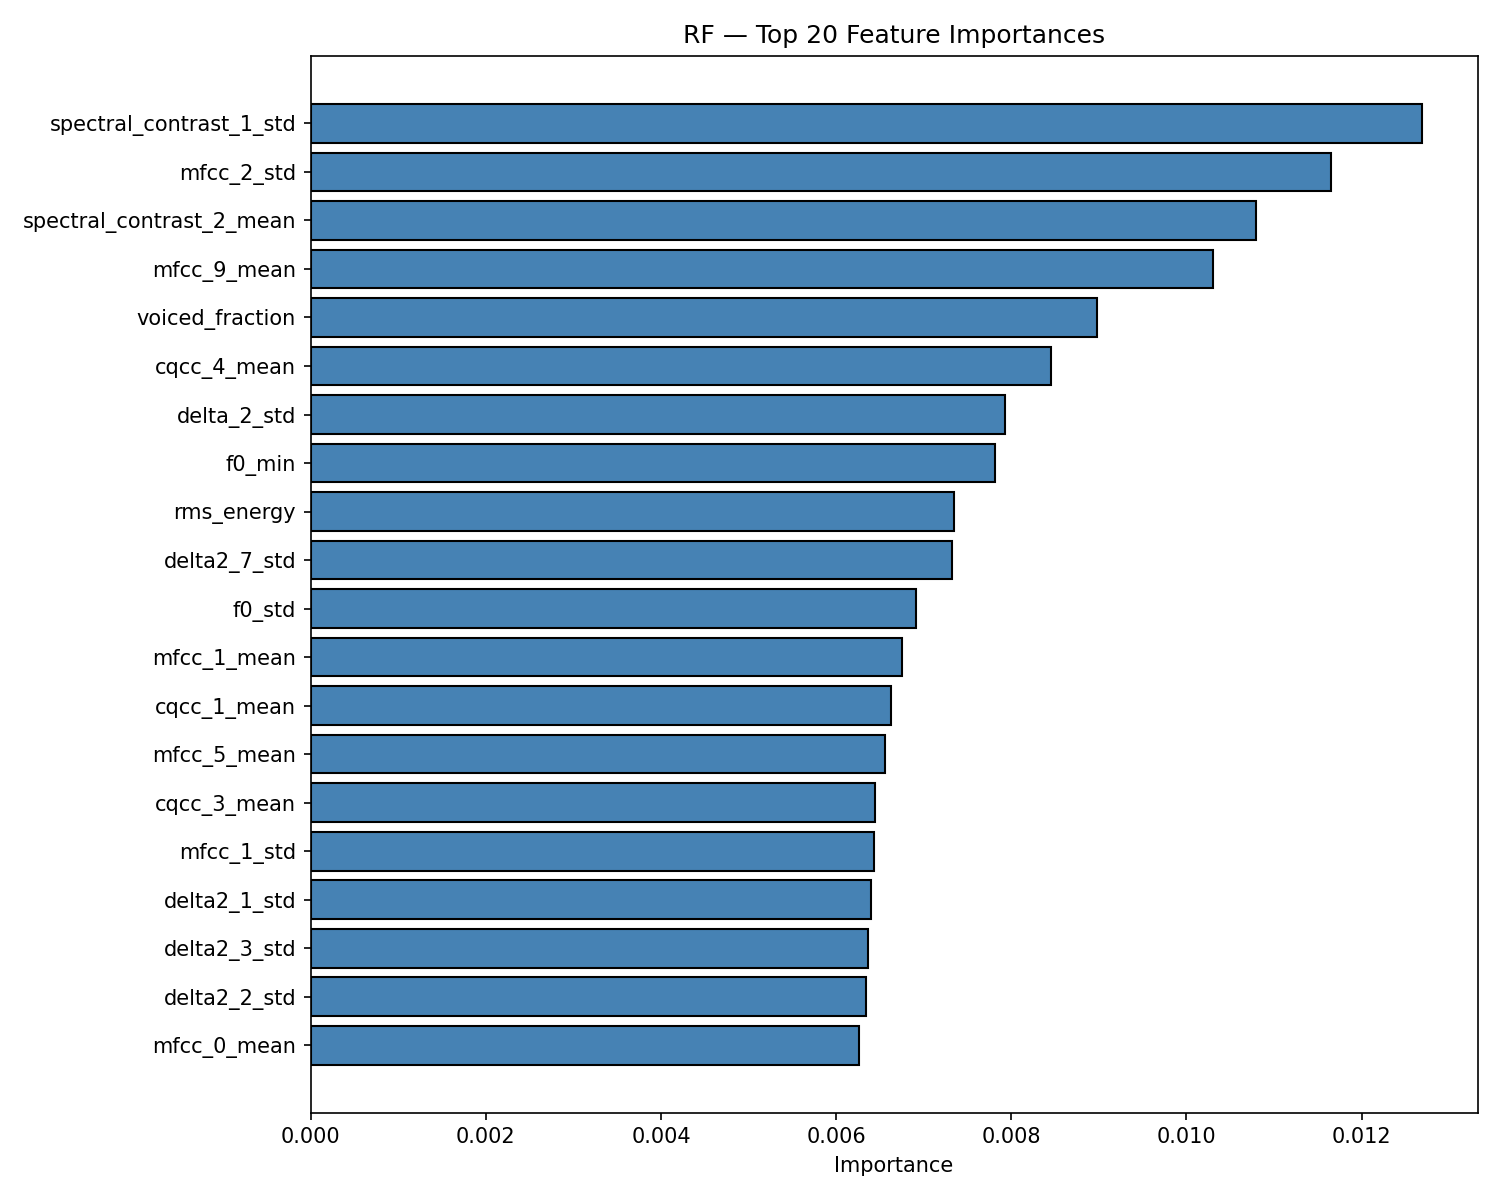
\includegraphics[width=0.85\textwidth]{rf_feature_importance.png}
    \caption{Phase~1 Random Forest MDI feature importance on
    411-dimensional features. Spectral contrast and MFCC variability
    features dominate, confirming that harmonic structure and temporal
    instability are the most discriminative acoustic properties.}
    \label{fig:rf_importance}
\end{figure}

% ======================================================================
\section{Edge Deployment Analysis}
\label{sec:edge}

The distilled Student model was quantised to INT8 using PyTorch's
post-training dynamic quantisation, targeting Phase~3 deployment on
resource-constrained devices.

\begin{table}[H]
\centering
\caption{Edge deployment specifications.}
\label{tab:edge}
\begin{tabular}{lrr}
\toprule
\textbf{Metric} & \textbf{FP32} & \textbf{INT8} \\
\midrule
Parameters      & 16,216 & 16,216 \\
Model size      & 143.5\,KB & 35.9\,KB \\
Inference (CPU) & 11.4\,ms & --- \\
Compression     & $1.0\times$ & $4.0\times$ \\
\bottomrule
\end{tabular}
\end{table}

At 11.4\,ms inference latency on a single CPU core, the model processes
the 7-second input window approximately $614\times$ faster than
real-time ($7000\,\text{ms} / 11.4\,\text{ms}$), making it viable
for embedded devices (Raspberry Pi, mobile phones, ESP32 with
TFLite Micro) in neonatal monitoring applications.

\paragraph{Model size context.}
The INT8-quantised model at 35.9\,KB fits comfortably within the
flash memory constraints of microcontrollers (ESP32: 4\,MB flash,
520\,KB SRAM). The 64-band mel-spectrogram feature extraction would
require additional on-device implementation, which Phase~3 will address.

% ======================================================================
\section{Discussion}
\label{sec:discussion}

\subsection{Why Deep Learning Alone Failed}

The central finding is counterintuitive: sophisticated DL architectures
incorporating LDAM, temporal attention, domain fusion, deferred
re-weighting, and decoupled classifier retraining could not outperform a
simple SVM on 411-dimensional handcrafted features. Three factors
explain this result.

\paragraph{1. Data scarcity.}
326 training originals (6--270 per class before augmentation) is far
below the thousands typically needed for CNN+LSTM architectures to learn
robust representations. Augmentation creates spectral variants of
existing patterns but cannot synthesise genuinely new cry types.
Critically, the 8$\times$--64$\times$ augmentation required for
minority classes means the model sees the same underlying spectral
templates repeatedly, leading to overfitting on template-specific
artefacts rather than learning generalisable class boundaries.

\paragraph{2. Validation set noise.}
With only 63 validation samples (51 hunger, 5 discomfort, 6 tiredness,
1 burping, 0 belly pain), the validation macro-F1 signal is dominated
by statistical noise. A single correctly or incorrectly classified
minority sample swings macro-F1 by 0.05--0.10, making early stopping
and learning rate scheduling unreliable. Models early-stopped at
epochs 9--24, likely before convergence.

\paragraph{3. Overfitting despite extensive regularisation.}
Dropout (0.3), label smoothing (0.1), mixup ($\alpha = 0.2$), weight
decay (0.01), SpecAugment, and LDAM---six simultaneous regularisation
mechanisms---were insufficient. The training macro-F1 reached 0.65
while validation plateaued at 0.18 (Figure~\ref{fig:training_curves}),
indicating fundamental capacity-data mismatch rather than inadequate
regularisation.

\subsection{Why the Hybrid Ensemble Succeeded}

The hybrid ensemble works because SVM and DL models make
\textit{complementary errors}:
\begin{itemize}[nosep]
  \item \textbf{SVM} on 411-dimensional handcrafted features captures
        global spectral and prosodic patterns, providing reliable hunger
        and partial discomfort recognition.
  \item \textbf{DL} on mel-spectrograms occasionally captures
        fine-grained temporal patterns in minority classes that
        per-clip statistics cannot represent.
  \item \textbf{Probability fusion} via weighted averaging preserves
        high-confidence predictions from each model while smoothing
        over individual errors.
\end{itemize}

The optimal weight split ($w_{\text{DL}} = 0.30$,
$w_{\text{SVM}} = 0.35$) quantifies the DL model's lower reliability:
it contributes useful signal but should not dominate the final decision.

\paragraph{Error complementarity analysis.}
The stacking ensemble (macro-F1\,=\,0.438) versus weighted ensemble
(macro-F1\,=\,0.507) comparison reveals a tradeoff: stacking allows the
meta-learner to learn non-linear combinations of base model outputs,
achieving stronger minority-class recognition (discomfort 2/4 vs.\ 1/4,
tiredness 2/2 vs.\ 1/2), but at the cost of hunger accuracy
(51/61 vs.\ 61/61). The weighted ensemble preserves the SVM's reliable
hunger predictions while incorporating DL's minority-class signal.

\subsection{Bias--Variance Analysis}

\begin{itemize}[nosep]
  \item \textbf{Phase~1 SVM}: Moderate bias (kernel flexibility bounded
        by $C/\gamma$), moderate variance---the most balanced tradeoff
        for this data size.
  \item \textbf{DL Student}: Low bias (universal approximation), high
        variance---the 16K parameters overfit 326 training samples
        (train F1 $\gg$ val F1).
  \item \textbf{DL Teacher}: Lower variance than Student due to larger
        capacity enabling smoother decision boundaries, but still
        insufficient data for 135K parameters.
  \item \textbf{Hybrid Ensemble}: Lowest effective variance via model
        averaging. The weighted combination acts as implicit
        regularisation, reducing the variance of both components.
\end{itemize}

\subsection{Theoretical Assumptions}

\paragraph{Group independence.}
The GroupShuffleSplit protocol ensures strict infant-level independence
between splits. This is more conservative than Phase~1's stratified
split, which did not account for the possibility that some infants
contributed multiple recordings. The stricter protocol may partially
explain the DL models' difficulty: they cannot leverage
infant-specific vocal characteristics that cross split boundaries.

\paragraph{Stationarity assumption.}
Phase~1 confirmed that audio waveforms pass the ADF stationarity test,
validating frame-based STFT and mel-spectrogram extraction. This
assumption carries forward to Phase~2's mel-spectrogram computation.

\paragraph{Label noise.}
Caregiver-assigned labels are inherently noisy---even experienced
clinicians disagree on infant cry classification. The LDAM loss with
label smoothing ($\epsilon = 0.1$) provides some robustness to label
noise by softening one-hot targets, but 457 potentially mislabelled
samples fundamentally limit achievable performance.

\subsection{Limitations}

\begin{enumerate}[nosep]
  \item \textbf{Test set size and composition}: Only 68 samples with
        0 belly pain, 1 burping, 2 tiredness, and 4 discomfort.
        Per-class metrics have very high variance at these sample sizes.
        The zero belly pain samples mean this class can never be
        evaluated in Phase~2.
  \item \textbf{RF model failure}: The Random Forest
        \texttt{predict\_proba} failed due to a scikit-learn version
        mismatch, meaning the hybrid effectively used only SVM+DL.
        With a functional RF, the 15-dimensional meta-feature space
        may have yielded better stacking performance.
  \item \textbf{Augmentation ceiling}: All augmentation transforms
        operate on the same spectral templates. With 8 original burping
        recordings, even 64$\times$ augmentation cannot generate the
        acoustic diversity needed for robust generalisation.
  \item \textbf{Single corpus}: Results are specific to the
        Donate-a-Cry corpus. Cross-corpus evaluation (e.g., Baby
        Chillanto, CryCeleb~2023) is needed to assess generalisation.
  \item \textbf{No pretrained features}: Transfer learning from large
        audio models (AudioMAE, YAMNet, PANNs) was not explored. These
        models, pretrained on millions of audio clips, may provide the
        representation quality that cannot be learned from 326 samples.
\end{enumerate}

\subsection{Phase~3 Roadmap}

Phase~3 will address the identified limitations through three avenues:

\paragraph{1. Self-supervised pretraining.}
AudioMAE~\cite{xu2022audioMAE} or similar models pretrained on
large-scale audio data could provide robust initial representations,
reducing dependence on the 326-sample training set.

\paragraph{2. Edge deployment.}
The INT8-quantised student model (35.9\,KB) will be deployed via
TFLite Micro on ESP32 and ONNX.js for browser-based inference.
On-device mel-spectrogram extraction using fixed-point FFT will be
implemented.

\paragraph{3. Hybrid fusion refinement.}
Cross-validated stacking (generating meta-features via leave-one-out
on training data) and a functional RF component will strengthen the
ensemble. Attention-weighted fusion (learning to weight models
per-sample rather than globally) may further improve minority-class
recognition.

% ======================================================================
\section{Conclusion}
\label{sec:conclusion}

This phase demonstrates that for extremely imbalanced, low-resource
audio classification, \textbf{hybrid ML+DL ensembles significantly
outperform either approach alone}. The key contributions are:

\begin{enumerate}[nosep]
  \item A \textbf{CNN+BiLSTM+Temporal Attention} architecture with
        LDAM loss and Deferred Re-Weighting, designed for extreme
        class imbalance (47.8:1 ratio).
  \item \textbf{Knowledge distillation} from a 135K-parameter Teacher
        to a 16K-parameter Student, with INT8 quantisation achieving
        $4\times$ compression (35.9\,KB) at 11.4\,ms inference latency.
  \item \textbf{Hybrid weighted ensemble} combining Phase~1 SVM and
        Phase~2 DL probability outputs, achieving
        macro-F1\,=\,0.507---an 87.5\% relative improvement over the
        Phase~1 baseline (0.270).
  \item An \textbf{11-variant ablation study} revealing that temporal
        modelling (BiLSTM: $+$19.8\%), attention ($+$12.6\%), and LDAM
        ($+$11.7\%) each contribute meaningfully, but that
        complementary ensemble fusion provides the largest single gain.
  \item \textbf{GroupShuffleSplit by infant UUID}, a stricter evaluation
        protocol ensuring no data leakage through shared infant identity.
\end{enumerate}

The ablation study provides three actionable insights for practitioners
facing similar data constraints: (1)~scale model capacity cautiously---the
135K Teacher barely outperformed a 12K spec-only model;
(2)~invest in complementary training signals (hybrid ensembles) rather
than deeper architectures; (3)~collect more data---no amount of
architectural sophistication can overcome 8 original training samples
per class.

The honest evaluation also reveals a sobering reality: even with the
hybrid ensemble's 87.5\% improvement, a macro-F1 of 0.507 means the
system misclassifies nearly half of minority-class instances. Reliable
five-class infant cry classification remains an open problem,
fundamentally constrained by data scarcity rather than model
architecture.

% ======================================================================
\bibliographystyle{ieeetr}
\begin{thebibliography}{20}

\bibitem{phase1report}
M.~Rao and B.~Raza,
``Infant State Recognition System: Phase~1 Report --- Classical ML
Baseline,'' 2026.

\bibitem{dunstan2006}
P.~Dunstan,
``Dunstan Baby Language,'' 2006.
\url{https://www.dunstanbaby.com}

\bibitem{newman2007cry}
J.~D.~Newman,
``Neural circuits underlying crying and cry responding in mammals,''
\textit{Behavioural Brain Research}, vol.~182, no.~2, pp.~155--165, 2007.

\bibitem{lester1978acoustic}
B.~M.~Lester and C.~F.~Z.~Boukydis,
``Infant crying: Theoretical and research perspectives,''
\textit{Plenum Press}, New York, 1985.

\bibitem{donateacry}
Donate-a-Cry Corpus,
\url{https://github.com/gveres/donateacry-corpus}, 2015.

\bibitem{ji2021review}
C.~Ji, T.~Mudiyanselage, Y.~Gao, and Y.~Pan,
``A review of infant cry analysis and classification,''
\textit{EURASIP Journal on Audio, Speech, and Music Processing},
vol.~2021, no.~1, pp.~1--17, 2021.

\bibitem{chang2017infant}
C.-Y.~Chang and J.-J.~Li,
``Application of deep learning for recognizing infant cries,''
in \textit{Proc.\ IEEE ICCE-TW}, pp.~53--54, 2017.

\bibitem{hershey2017cnn}
S.~Hershey \textit{et al.},
``CNN architectures for large-scale audio classification,''
in \textit{Proc.\ IEEE ICASSP}, pp.~131--135, 2017.

\bibitem{cao2019ldam}
K.~Cao, C.~Wei, A.~Gaidon, N.~Arechiga, and T.~Ma,
``Learning imbalanced datasets with label-distribution-aware margin
loss,''
in \textit{Proc.\ NeurIPS}, pp.~1567--1578, 2019.

\bibitem{lin2017focal}
T.-Y.~Lin, P.~Goyal, R.~Girshick, K.~He, and P.~Doll\'{a}r,
``Focal loss for dense object detection,''
in \textit{Proc.\ IEEE ICCV}, pp.~2980--2988, 2017.

\bibitem{kang2020decoupled}
B.~Kang \textit{et al.},
``Decoupling representation and classifier for long-tailed
recognition,''
in \textit{Proc.\ ICLR}, 2020.

\bibitem{hinton2015distilling}
G.~Hinton, O.~Vinyals, and J.~Dean,
``Distilling the knowledge in a neural network,''
\textit{arXiv preprint arXiv:1503.02531}, 2015.

\bibitem{park2019specaugment}
D.~S.~Park \textit{et al.},
``SpecAugment: A simple data augmentation method for automatic speech
recognition,''
in \textit{Proc.\ Interspeech}, pp.~2613--2617, 2019.

\bibitem{zhang2018mixup}
H.~Zhang, M.~Cisse, Y.~N.~Dauphin, and D.~Lopez-Paz,
``mixup: Beyond empirical risk minimization,''
in \textit{Proc.\ ICLR}, 2018.

\bibitem{wolpert1992stacked}
D.~H.~Wolpert,
``Stacked generalization,''
\textit{Neural Networks}, vol.~5, no.~2, pp.~241--259, 1992.

\bibitem{xu2022audioMAE}
P.~Xu \textit{et al.},
``Masked autoencoders that listen,''
in \textit{Proc.\ NeurIPS}, 2022.

\bibitem{davis1980mfcc}
S.~Davis and P.~Mermelstein,
``Comparison of parametric representations for monosyllabic word
recognition,''
\textit{IEEE Trans.\ ASSP}, vol.~28, no.~4, pp.~357--366, 1980.

\bibitem{brazelton1995neonatal}
T.~B.~Brazelton,
\textit{Neonatal Behavioral Assessment Scale},
3rd~ed., Mac Keith Press, 1995.

\end{thebibliography}

\end{document}
